\documentclass[a4paper,11pt]{article}
\usepackage{graphicx}
\usepackage{float}
\usepackage{subfig}
\usepackage{geometry}
\usepackage{amsmath,amssymb}
\usepackage{amsthm}
\usepackage{bbold}
\usepackage{mathtools}
\usepackage{braket}
\usepackage{booktabs}
\usepackage[table,xcdraw]{xcolor}
\usepackage[utf8]{inputenc}
\usepackage{cite}
\usepackage[english]{babel}
\usepackage{lipsum}
\usepackage{setspace}
\usepackage{minted}
\usepackage{xcolor}
\newcommand{\R}{\mathbb{R}}
\usepackage{hyperref}
\hypersetup{colorlinks=true,linkcolor=blue}
\geometry{a4paper, top=2.5cm, bottom=2.5cm, left=3cm, right=2.5cm}

\begin{document}
	\author{Catalano Giuseppe, Cerrato Nunzia}
	\title{Numerical Linear Algebra Homework Project 2:\\Least Squares, Orthogonalization, and the SVD}
	\date{}
	\maketitle
	
\section*{Problem 3}	
\noindent \textbf{(1)} Let $A \in \R^{m\times n}$, with $\text{rank}(A) = n$. The singular value decomposition of $A$ can be written as $A = U \Sigma V^T$ or, equivalently, as $A = \sum_{i=1}^n \sigma_i \textbf{u}_i \textbf{v}_i^T$, where $\sigma_1 \ge \sigma_2 \ge \dots \ge \sigma_n$ represent the singular values of $A$, while $\{\textbf{u}_{i}\}_{i=1,\dots,n}$ and $\{\textbf{v}_{i}\}_{i=1,\dots,n}$ are, respectively, left and right singular vectors of $A$.\\

\noindent Express the singular values and singular vectors of the following matrices in terms of those of $A$.\\

\noindent \textbf{(a)} {$(A^{T}A)^{-1}$}
\[(A^{T}A)^{-1} = (V^{T})^{-1}\Sigma^{-2}V^{-1}=V\Sigma^{-2}V^{T}\]
In order to obtain this expression we used that $U^{T}U=\mathbb{1}$ and that $V^{-1}=V^{T}$, since $U$ and $V$ are orthogonal. We can conclude that both left and right singular vectors of $(A^{T}A)^{-1}$ are equal to the right singular vectors of $A$, while singular values of the former matrix are equal to those of $A$ raised to the $-2$ power. Note that, since singular values of $A$ are in increasing order and in this expression they are raised to a negative power, they must appear in reverse order.\\

%\begin{itemize}
%	\item Both left and right singular vectors of $(A^{T}A)^{-1}$ are equal to the right singular vectors of $A$;
%	\item Singular values of $(A^{T}A)^{-1}$ are equal to singular values of $A$ raised to the $-2$ power.
%\end{itemize}

\noindent \textbf{(b)} $(A^{T}A)^{-1}A^{T}$
\[(A^{T}A)^{-1}A^{T} = V\Sigma^{-2}V^{T}V\Sigma U^{T}=V\Sigma^{-1}U^{T}\]
Analogously to the previous case, we know that $V^{T}V=\mathbb{1}$. Here we see that left singular vectors of $(A^{T}A)^{-1}A^{T}$ are equal to the right singular vectors of $A$, right singular vectors of $(A^{T}A)^{-1}A^{T}$ are equal to the left singular vectors of $A$, while singular values of this matrix are equal to the inverse of singular values of $A$.\\

%\begin{itemize}
%	\item Left singular vectors of $(A^{T}A)^{-1}A^{T}$ are equal to the right singular vectors of $A$;
%	\item Right singular vectors of $(A^{T}A)^{-1}$ are equal to the left singular vectors of $A$;
%	\item Singular values of $(A^{T}A)^{-1}$ are equal to the inverse of singular values of $A$.
%\end{itemize}

\noindent \textbf{(c)} $A(A^{T}A)^{-1}$
\[A(A^{T}A)^{-1} = U\Sigma V^{T}V\Sigma^{-2}V^{-T}=U\Sigma^{-1}V^{T}\]
Note that this result can also be obtained from the previous case, by noting that $A(A^{T}A)^{-1}=((A^{T}A)^{-1}A^{T})^{T}$. We can see that left and right singular vectors of $(A^{T}A)^{-1}$ coincide with that of $A$, while singular values of this matrix are equal to the inverse of singular values of $A$.\\
%\begin{itemize}
%	\item Left and right singular vectors of $(A^{T}A)^{-1}$ coincide with that of $A$;
%	\item Singular values of $(A^{T}A)^{-1}$ are equal to the inverse of singular values of $A$.
%\end{itemize}

\noindent \textbf{(d)} $A(A^{T}A)^{-1}A^{T}$
\[A(A^{T}A)^{-1}A^{T} = U\Sigma^{-1}V^{T}V\Sigma U^{T}= U U^{T} \]
In this case, both left and right singular vectors of $A(A^{T}A)^{-1}A^{T}$ are equal to left singular vectors of $A$, while singular values of this matrix are all equal to $1$.\\


\noindent \textbf{(2)} Given the following matrix:
\begin{equation}
	A = \begin{bmatrix}
		1 & 2 \\
		0 & 2
	\end{bmatrix},
\end{equation}
its singular values can be computed by considering the square root of the eigenvalues of the matrix $A^{T}A$, which has the form:
\begin{equation}
	A^{T}A = \begin{bmatrix}
		1 & 2 \\
		2 & 8
	\end{bmatrix}.
\end{equation}
Hence, by imposing that $p(\lambda)=\det(A^{T}A -\lambda\mathbb{1})=0$, we find the two eigenvalues of $A^{T}A$ and, therefore, the two singular values of $A$, which are:
\begin{equation}
	\sigma_{1,2}=\sqrt{\frac{9 \pm \sqrt{65}}{2}}.
\end{equation}
Finally, knowing that the spectral condition number is defined as $k_{2}(A) = \frac{\sigma_{\max}}{\sigma_{\min}}$, we can find the condition number of $A$:
\begin{equation}
	k_{2}(A) = \sqrt{\frac{9+\sqrt{65}}{9-\sqrt{65}}} \simeq 4.26.
\end{equation}
We want now to see how the unit ball is modified by the transformation described by the matrix $A$. In other words, we want to see what is the image of a vector $\textbf{x}=(\cos(\theta),\sin(\theta))$, parametrizing the unit ball on a plane, when considering the linear transformation $\textbf{y}=A\textbf{x}$. The vector $\textbf{y}$ under the transformation $A$ assumes the form:
\[\textbf{y}=(\cos(\theta) + 2\sin(\theta), 2\sin(\theta)) \quad \theta \in \left[0,2\pi\right).\]
Graphically, we have:
\begin{figure}[H]
	\centering
	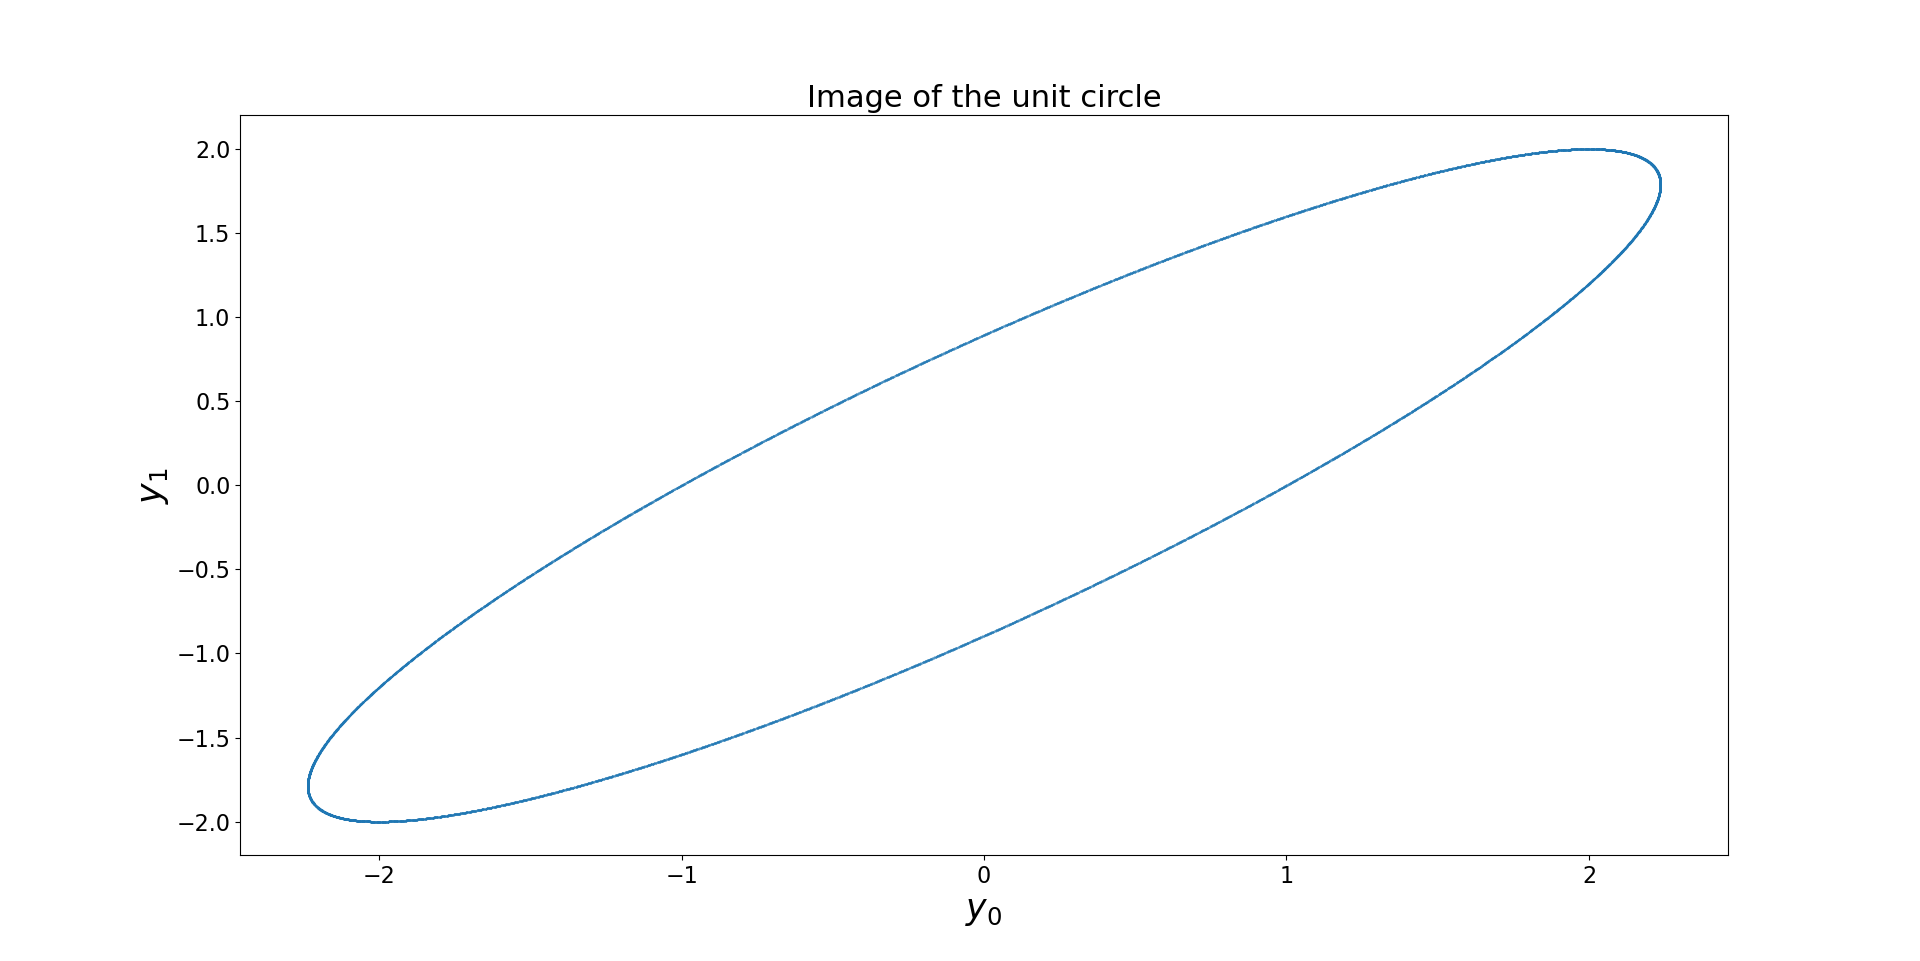
\includegraphics[scale=0.25]{Plot/Image_unit_circle}
	\caption{Image of the unit circle}
	\label{fig:Image_unit_circle}
\end{figure}

\noindent \textbf{(3)} jvejkvbkdjf\\


\noindent \textbf{(4)} Given a matrix
\begin{equation}
	A = \begin{bmatrix}
		-4 & -2 & -4 & -2 \\
		2 & -2 & 2 & 1 \\
		-800 & 200 & -800 & -401
	\end{bmatrix}.
\end{equation}
we want to compute the the singular values of $A$, the Moore-Penrose pseudoinverse of $A$ and its spectral condition number. We report in the following the Python script that we used to do it.

\begin{minted}[mathescape, linenos, breaklines]{python}
import numpy as np

A = np.array([[-4.,-2.,-4.,-2.],[2.,-2.,2.,1.],[-800,200,-800,-401]])
U, singular_values, V_transpose = np.linalg.svd(A, compute_uv=True)
pseudoinverse = np.linalg.pinv(A)
spectral_cond_num = np.linalg.cond(A)
print(f'singular values of A = {singular_values}')
print(f'pseudoinverse of A = {pseudoinverse}')
print(f'spectral condition number of A = {spectral_cond_num}')
\end{minted}

\noindent The results we obtained are reported below:

\begin{minted}{text}
singular values of A = [1.21689895e+03 3.30829410e+00 4.21538860e-03]
pseudoinverse of A = [[-2.50833333e+01  5.00833333e+01  2.50000000e-01]
                      [-1.66666667e-01 -3.33333333e-01  7.57226996e-16]
                      [-2.50833333e+01  5.00833333e+01  2.50000000e-01]
                      [ 1.00000000e+02 -2.00000000e+02 -1.00000000e+00]]
spectral condition number of A = 288680.1350686104
\end{minted}

\noindent Given the obtained results, we can say that $\text{rank}(A)=3$.\\

\noindent \textbf{(5)} The best rank-k approximation of a matrix $A$, in the Frobenius norm, is obtained by computing the singular value decomposition of $A$ and then by considering only the first $k$ terms in that expression. In other words, given a matrix $A$ written in terms of its singular value decomposition as $A = \sum_{i=1}^{n}\sigma_{i}\textbf{u}_{i}\textbf{v}_{i}^{T}$, its best rank-k approximation is given by $\tilde{A}_{k} = \sum_{i=1}^{k}\sigma_{i}\textbf{u}_{i}\textbf{v}_{i}^{T}$. Below is reported the Python code that we used to obtain the best rank-1 and rank-2 approximations of the matrix $A$ mentioned in the previous point of this exercise.

\begin{minted}[mathescape, linenos, breaklines]{python}
A_rank_1 = singular_values[0]*np.outer(U[:,0],V_transpose[0])
A_rank_2 = A_rank_1 + singular_values[1]*np.outer(U[:,1],V_transpose[1])
spectral_cond_num_A_rank_2 = singular_values[0]/singular_values[1]
print(f'A_rank_1 = {A_rank_1}')
print(f'A_rank_2 = {A_rank_2}')
print(f'Spectral condition number of A_rank_2 = {spectral_cond_num_A_rank_2}')
\end{minted}

\noindent We obtained the following two matrices:

\begin{minted}{text}
A_rank_1 = [[-3.67478811e+00  9.18652344e-01 -3.67478811e+00 -1.84198740e+00]
            [ 2.16152803e+00 -5.40355726e-01  2.16152803e+00  1.08346585e+00]
            [-8.00001057e+02  1.99990537e+02 -8.00001057e+02 -4.01000500e+02]]

A_rank_2 = [[  -3.99955481   -2.00000178   -3.99955481   -2.00177721]
            [   1.99910978   -1.99999645    1.99910978    1.00355377]
            [-800.00000445  200.00000002 -800.00000445 -400.99998223]]

Spectral condition number of A_rank_2 = 367.8327598758788
\end{minted}

\noindent As we can see, the best rank-1 approximation of $A$ returns a matrix that is already quite similar to the initial one, and the approximation improves when considering the best rank-2 approximation of $A$. This can be seen, in a more quantitative way, by considering the Frobenius norm of the difference between the approximated matrix and the initial matrix, both for the rank-1 and rank-2 approximation. By doing this, one obtains:

\begin{minted}{text}
Frobenious norm between A and A_rank_1 = 3.308296788282531
Frobenious norm between A and A_rank_2 = 0.004215388599497665
\end{minted}

\noindent \textbf{(6)} Consider an upper triangular matrix matrix $R = (r_{ij})$, whose entries are given by $r_{ii} = 1$ and $r_{ij} = -1$ for $j>i$. We defined a function \mintinline{python}{R_matrix(n)} that allows us to compute this matrix for a given dimension $n$:

\begin{minted}{python}
def R_matrix(n):
 R = np.triu(-np.ones((n,n)),k=1) + np.eye(n)
 return R
\end{minted}
Note that we used an upper triangular mask to obtain the entries $r_{ij}$. Once derived $R$, we computed its singular values for $n = 10,20,50,100$, as required. The plot of the singular values are reported below. 
\begin{figure}[H]
	\centering
	\subfloat[][n=10]{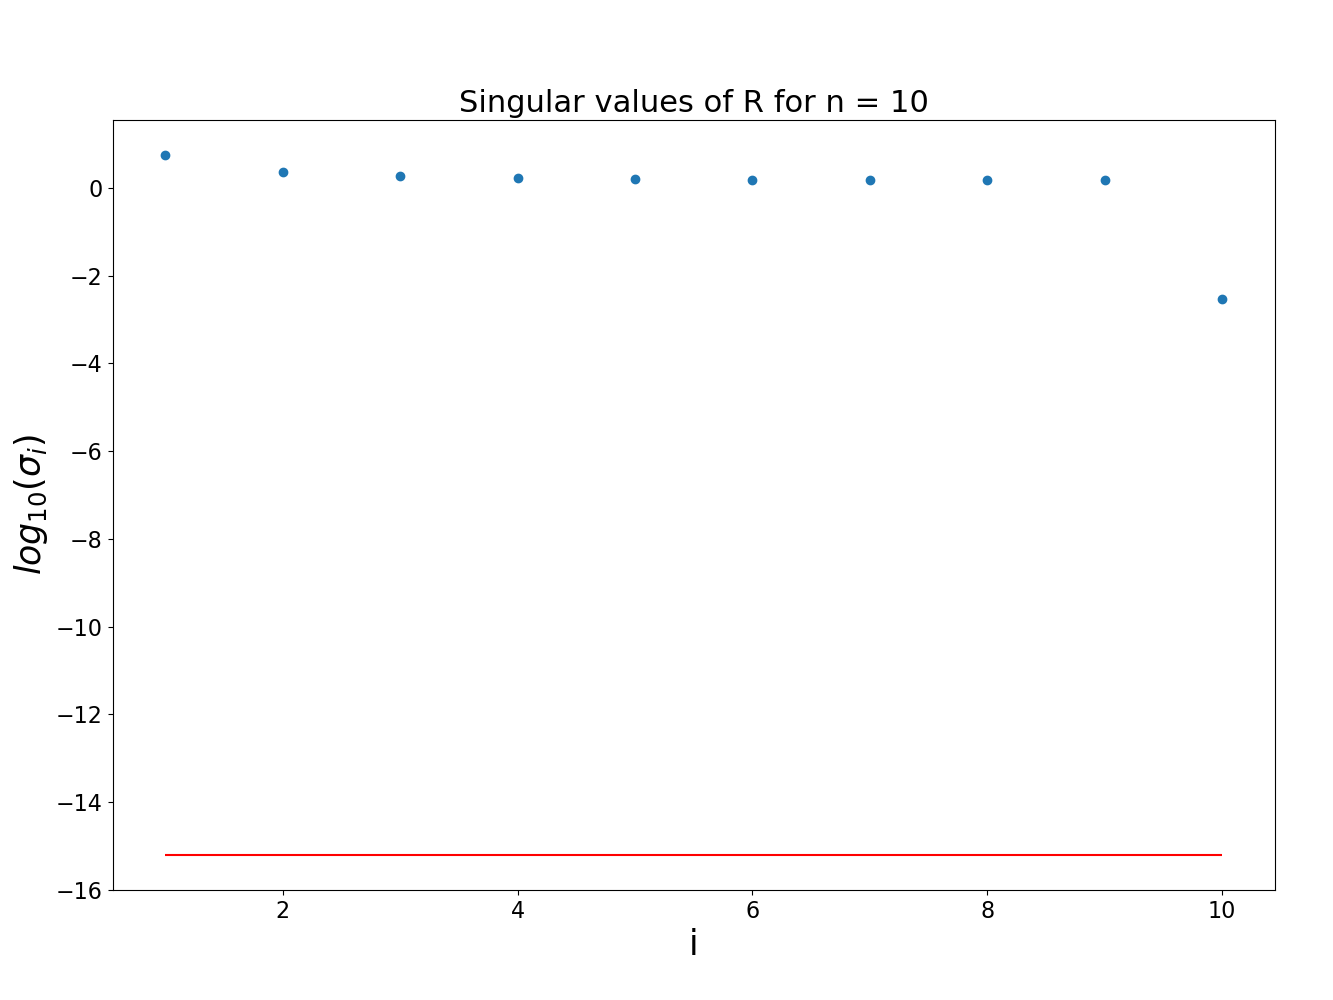
\includegraphics[scale=0.23]{Plot/Singular_values_of_R_for_n=10}} \qquad \subfloat[][n=20]{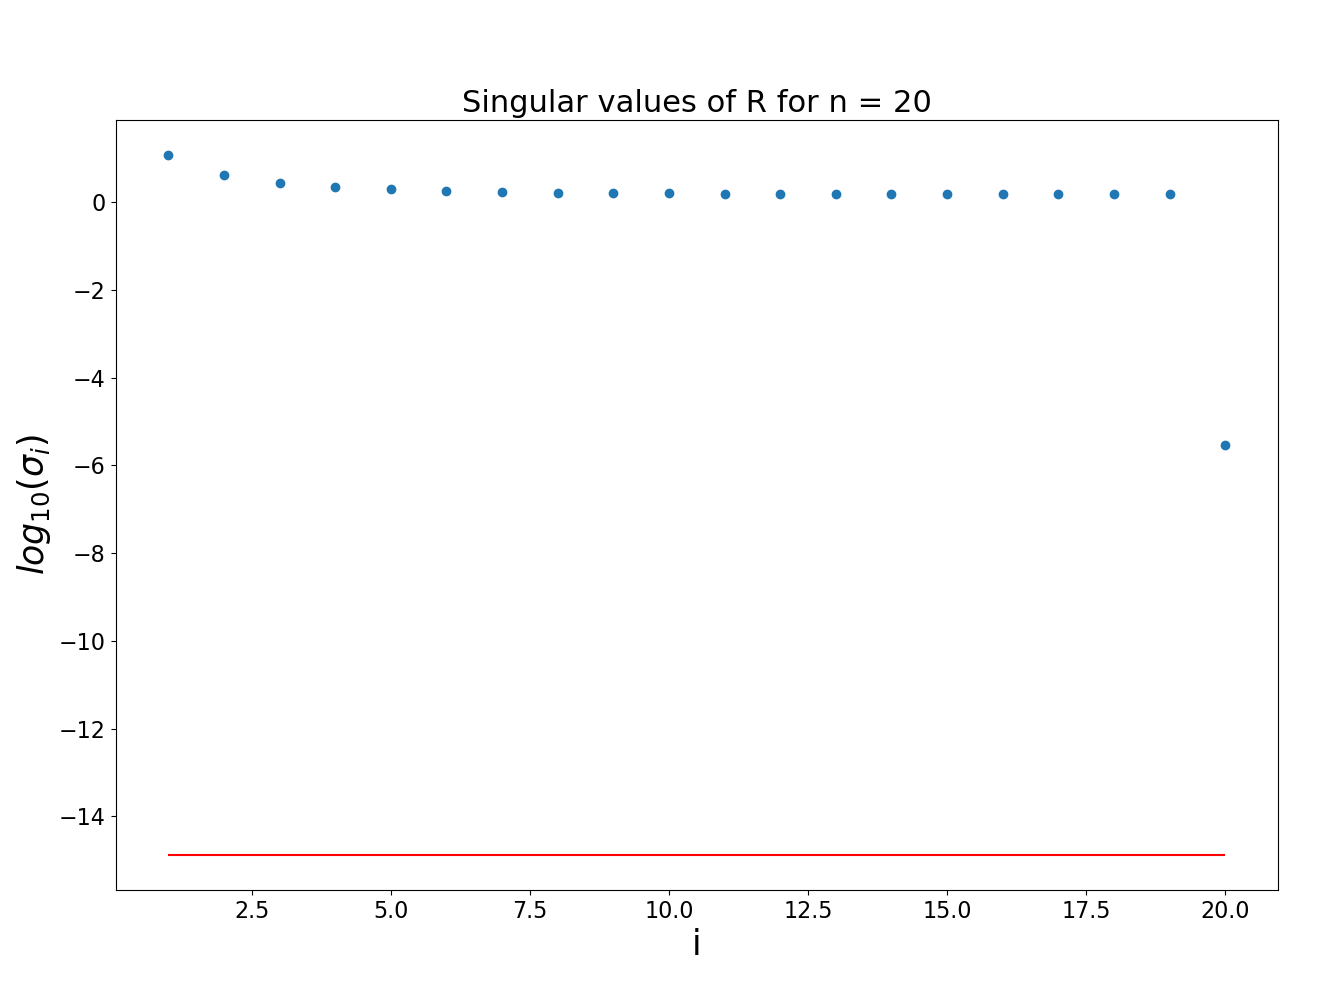
\includegraphics[scale=0.23]{Plot/Singular_values_of_R_for_n=20}} \\
	\subfloat[][n=50]{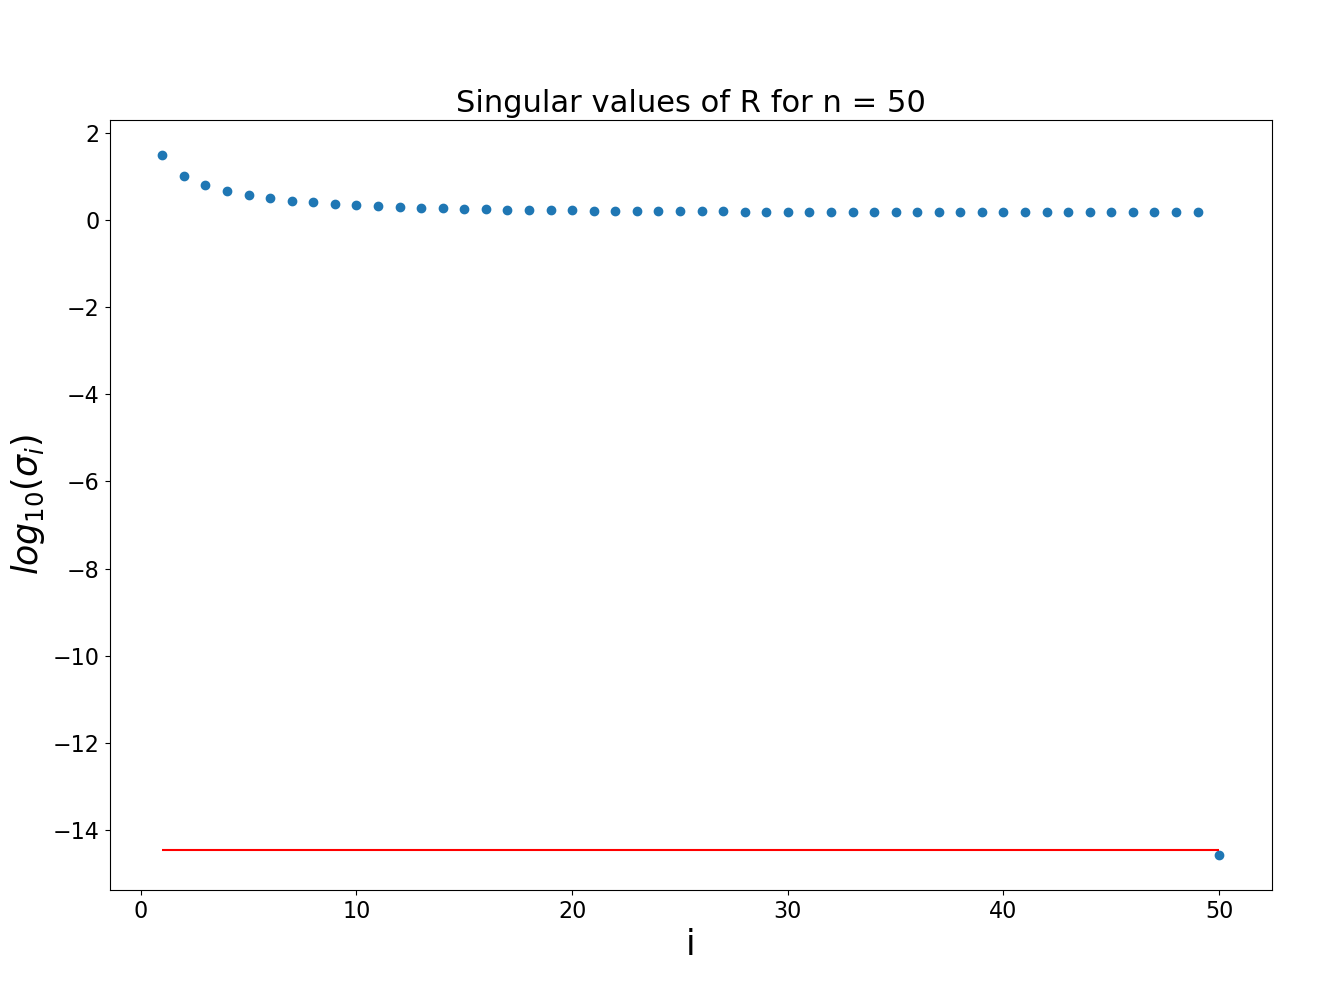
\includegraphics[scale=0.23]{Plot/Singular_values_of_R_for_n=50}} \qquad
	\subfloat[][n=100]{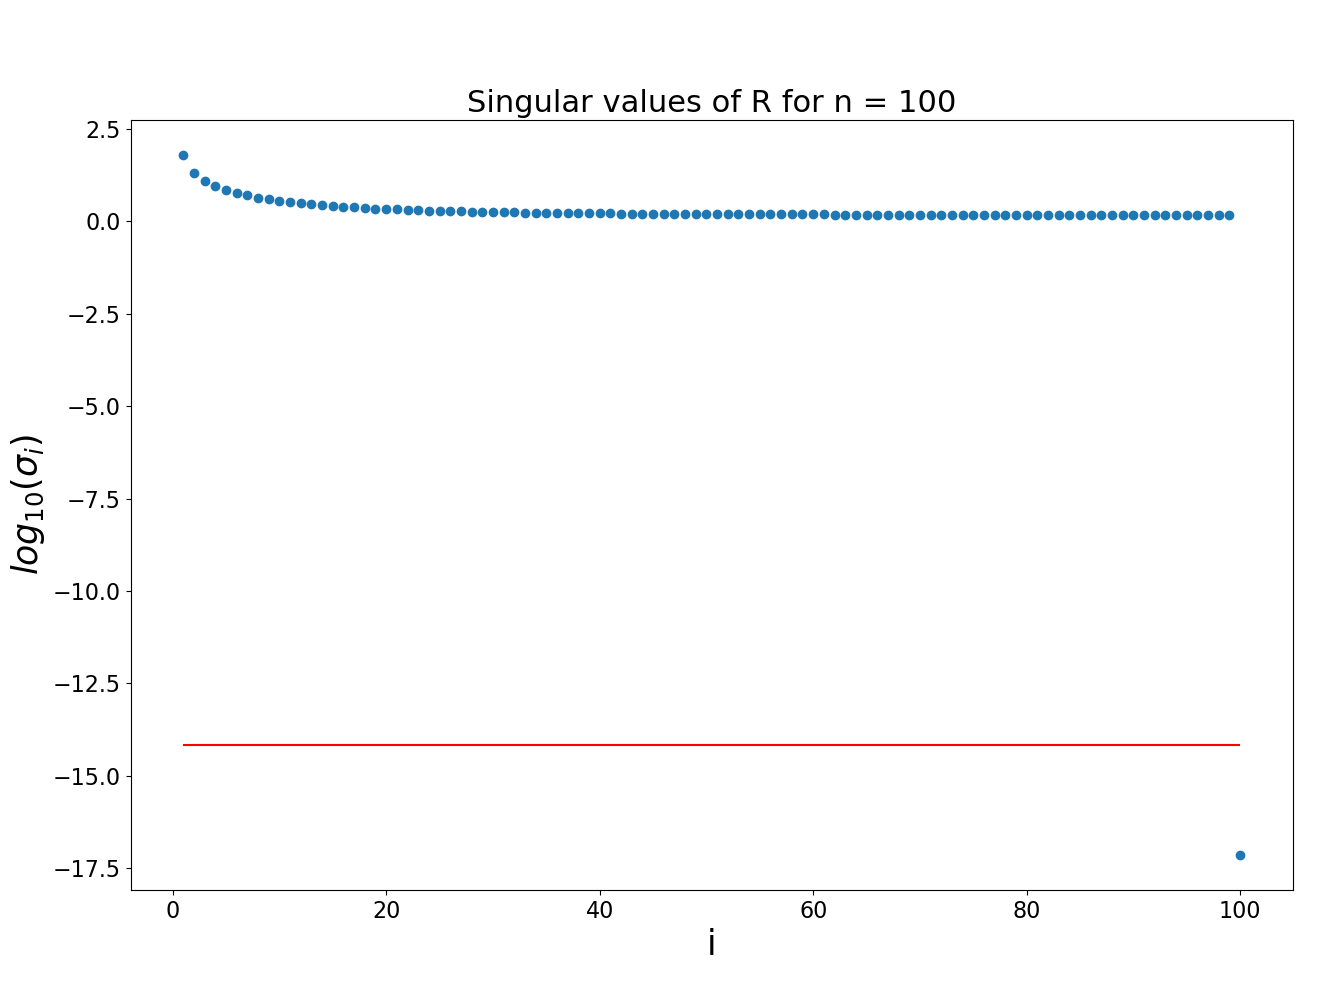
\includegraphics[scale=0.23]{Plot/Singular_values_of_R_for_n=100}}
	
	\caption{Singular values of the matrix $R$ defined at the beginning of this exercise for $n=10,20,50,100$.}
	\label{fig:Singular_values_of_R_for_different_dimensions}
\end{figure}

\noindent It can be observed that for $n=50$ and for $n=100$ the last singular value becomes smaller than the threshold value fixed by $u\sigma_{1}$, where $u$ is the machine precision. This means that, when this happens, the matrix $R$ becomes numerically singular.

\begin{figure}[H]
	\centering
	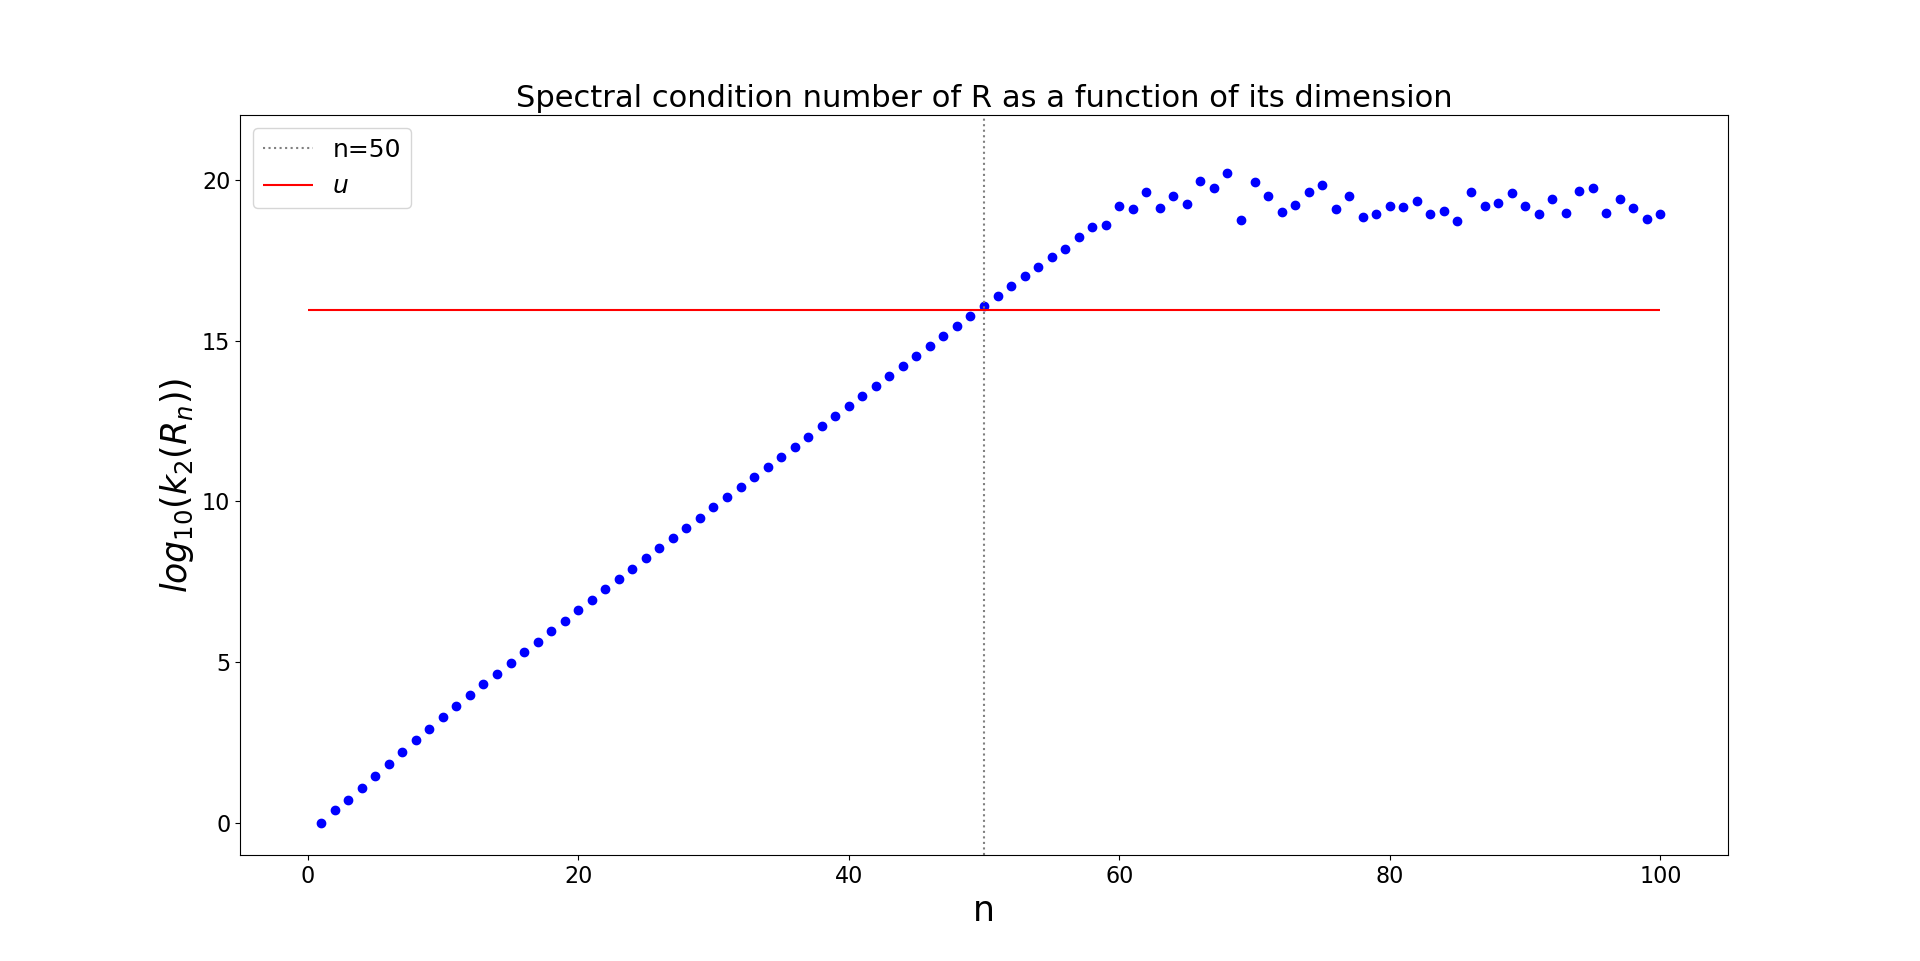
\includegraphics[scale=0.25]{Plot/Spectral_cond_num_R}
	\caption{Spectral condition number of $R$ as a function of its dimension.}
	\label{fig:Spectral_cond_num_R}
\end{figure}

	
	
\end{document}